This chapter provides an overview of the background and concepts related to this dissertation. Section~\ref{sec:text-localization-recognition}
introduces the main concepts related to text localization and recognition problem. Next, in Section~\ref{sec:deep-learning},  we briefly present a background on deep learning and on its use in the context of restricted computing power scenarios. Finally, examples of efficient and effective methods are discussed.

\section{Text Localization and Recognition}
\label{sec:text-localization-recognition}

Text localization and recognition in images and videos from diverse sources have received substantial attention recently, as diverse ``robust reading'' competitions as ICDAR'11 ~\cite{Karatzas2011ICDAR}, ICDAR'13~\cite{Karatzas2013ICDAR}, and ICDAR'15~\cite{icdar15} emerged as tools to infer the state-of-the-art in methods designed to address this issue.%\todo[inline]{I did not understand the message of this paragraph.}

%\textcolor{red}{Rewrite the paragraph below}
%The main objective can be summarized in determining if there is text in given image, detect it localize it then recognize it. 

The objectives of text localization and recognition are:
\begin{itemize}
    \item To determine if there is a text in a given image;
    \item To find the text location, obtaining the estimated position in the image; and %\todo{tell something about the expected output of this step}
    \item To recognize the text, obtaining the characters or words contained in the text.%\todo{tell something about the expected output of this step}
\end{itemize}

\subsection{Scene Text}
    Given the huge rise in the availability of portable, accessible image recorders as smartphones and cameras, it is possible to notice an equivalent increase in the size of data archives and datasets composed of images. A very common element in digital images is text. Text in digital images can occur in a variable fashion: as artificially generated graphic text, digitally added to an image as a caption; or even in scenarios related to giving some useful context to the image as a timestamp or subtitles; and in scene images, which is naturally found in the image captured by the camera and is part of the scene, like a shop facade or a street sign, for example. 
    
    Graphic, or born-digital images, as is called in ICDAR'11 competition~\cite{Karatzas2011ICDAR}, have some characteristics so that methods can take advantages of them. Commonly, born-digital images have the text horizontally oriented, in the foreground, with high contrast and in a very controlled background. Examples of such images can be found in Figure~\ref{fig:sample_icdar11}. Scene text, as shown in Figure~\ref{fig:sample_icdar13}, is a lot more complex: the text is usually cluttered with the background, with variable texture, color, illumination and orientation. Furthermore, possible deformations derived from a perspective view and occlusions from other objects can also be found.
    %\todo[inline]{Please check if you added a period in every caption in the dissertation}
    \begin{figure}[h!]
    \centering
	
\includegraphics[height=0.19\textheight]{dataset_samples/icdar11/img_40.jpg}
	
\includegraphics[height=0.19\textheight]{related_work/figs/icdar11_img_33.png}
	
\includegraphics[height=0.19\textheight]{related_work/figs/icdar11_img_30.png}

	\vspace{1.5mm}
	
	
\includegraphics[height=0.16\textheight]{dataset_samples/icdar11/img_138.jpg}
	
\includegraphics[height=0.16\textheight]{dataset_samples/icdar11/img_89.jpg}
	
\includegraphics[height=0.16\textheight]{related_work/figs/icdar11_img_64.jpg}

	
	
	\caption{Examples of images with digitally generated text (extracted from the ICDAR'11 dataset~\cite{Karatzas2011ICDAR}).}
	\label{fig:sample_icdar11}
    \end{figure}

    \begin{figure}[h!]
        \centering
    	
\includegraphics[height=0.18\textheight]{related_work/figs/icdar13_img_8.jpg}
    	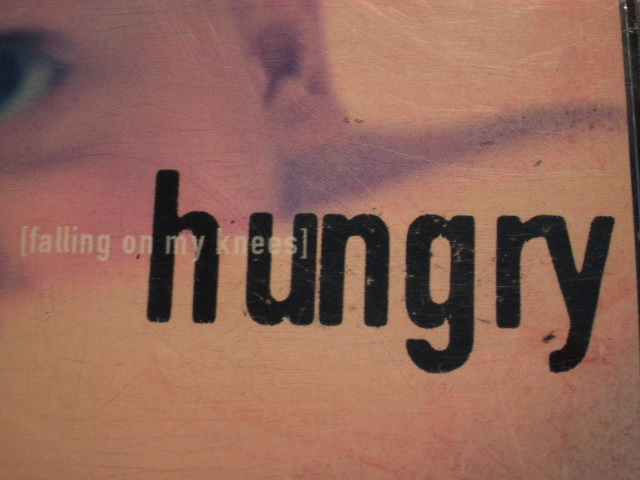
\includegraphics[height=0.18\textheight]{related_work/figs/icdar13_img_5.jpg}
    	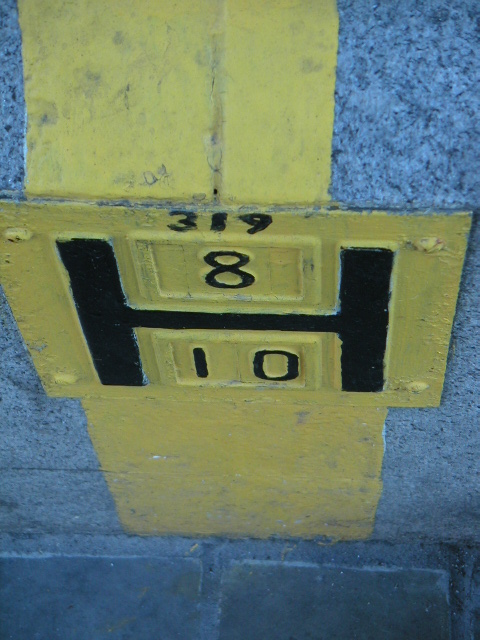
\includegraphics[height=0.18\textheight]{related_work/figs/icdar13_img_2.jpg}
    
    	\vspace{1.5mm}
    	
    	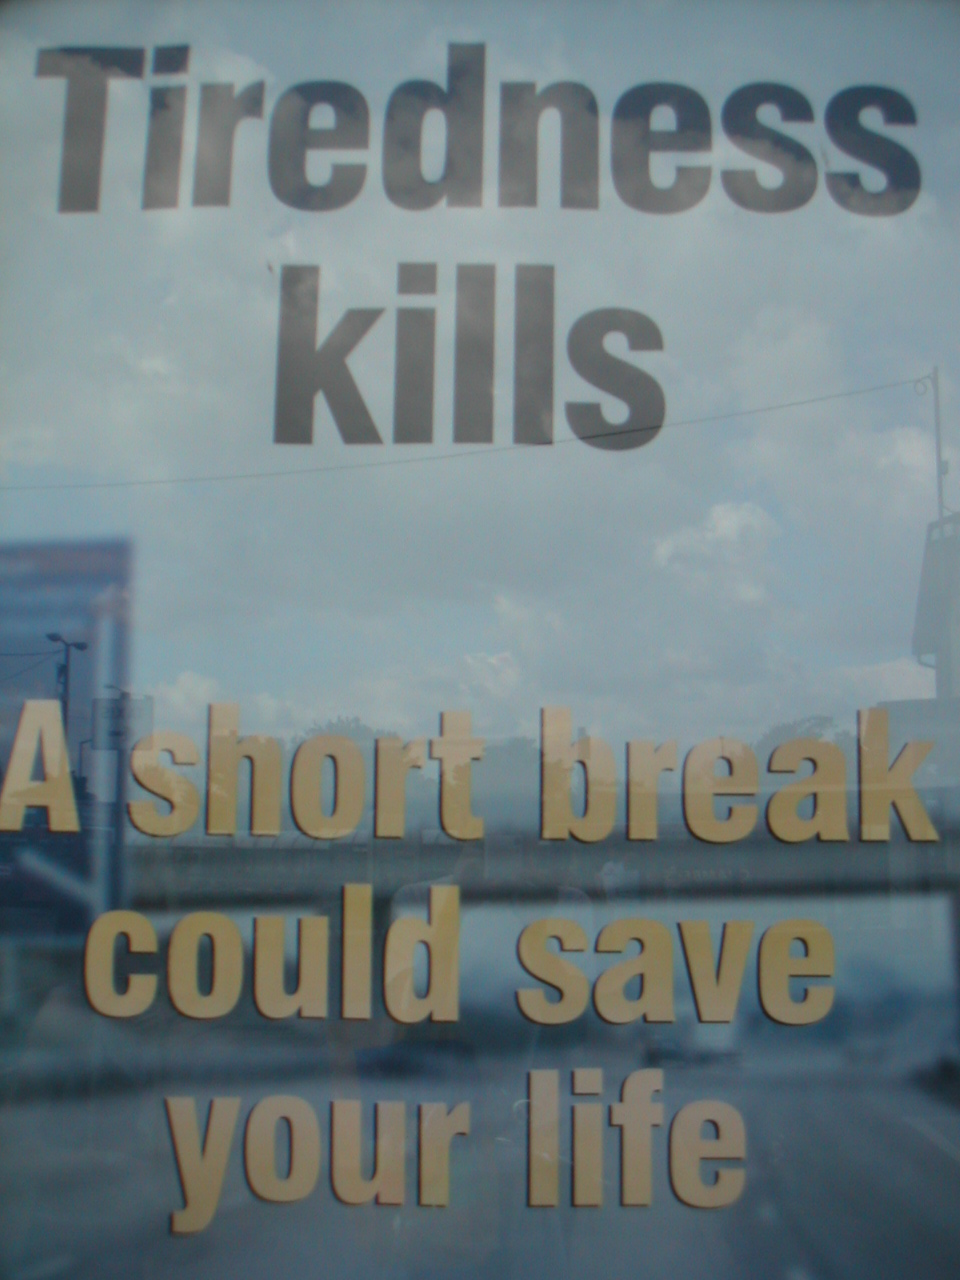
\includegraphics[height=0.172\textheight]{related_work/figs/icdar13_img_1.jpg}
    	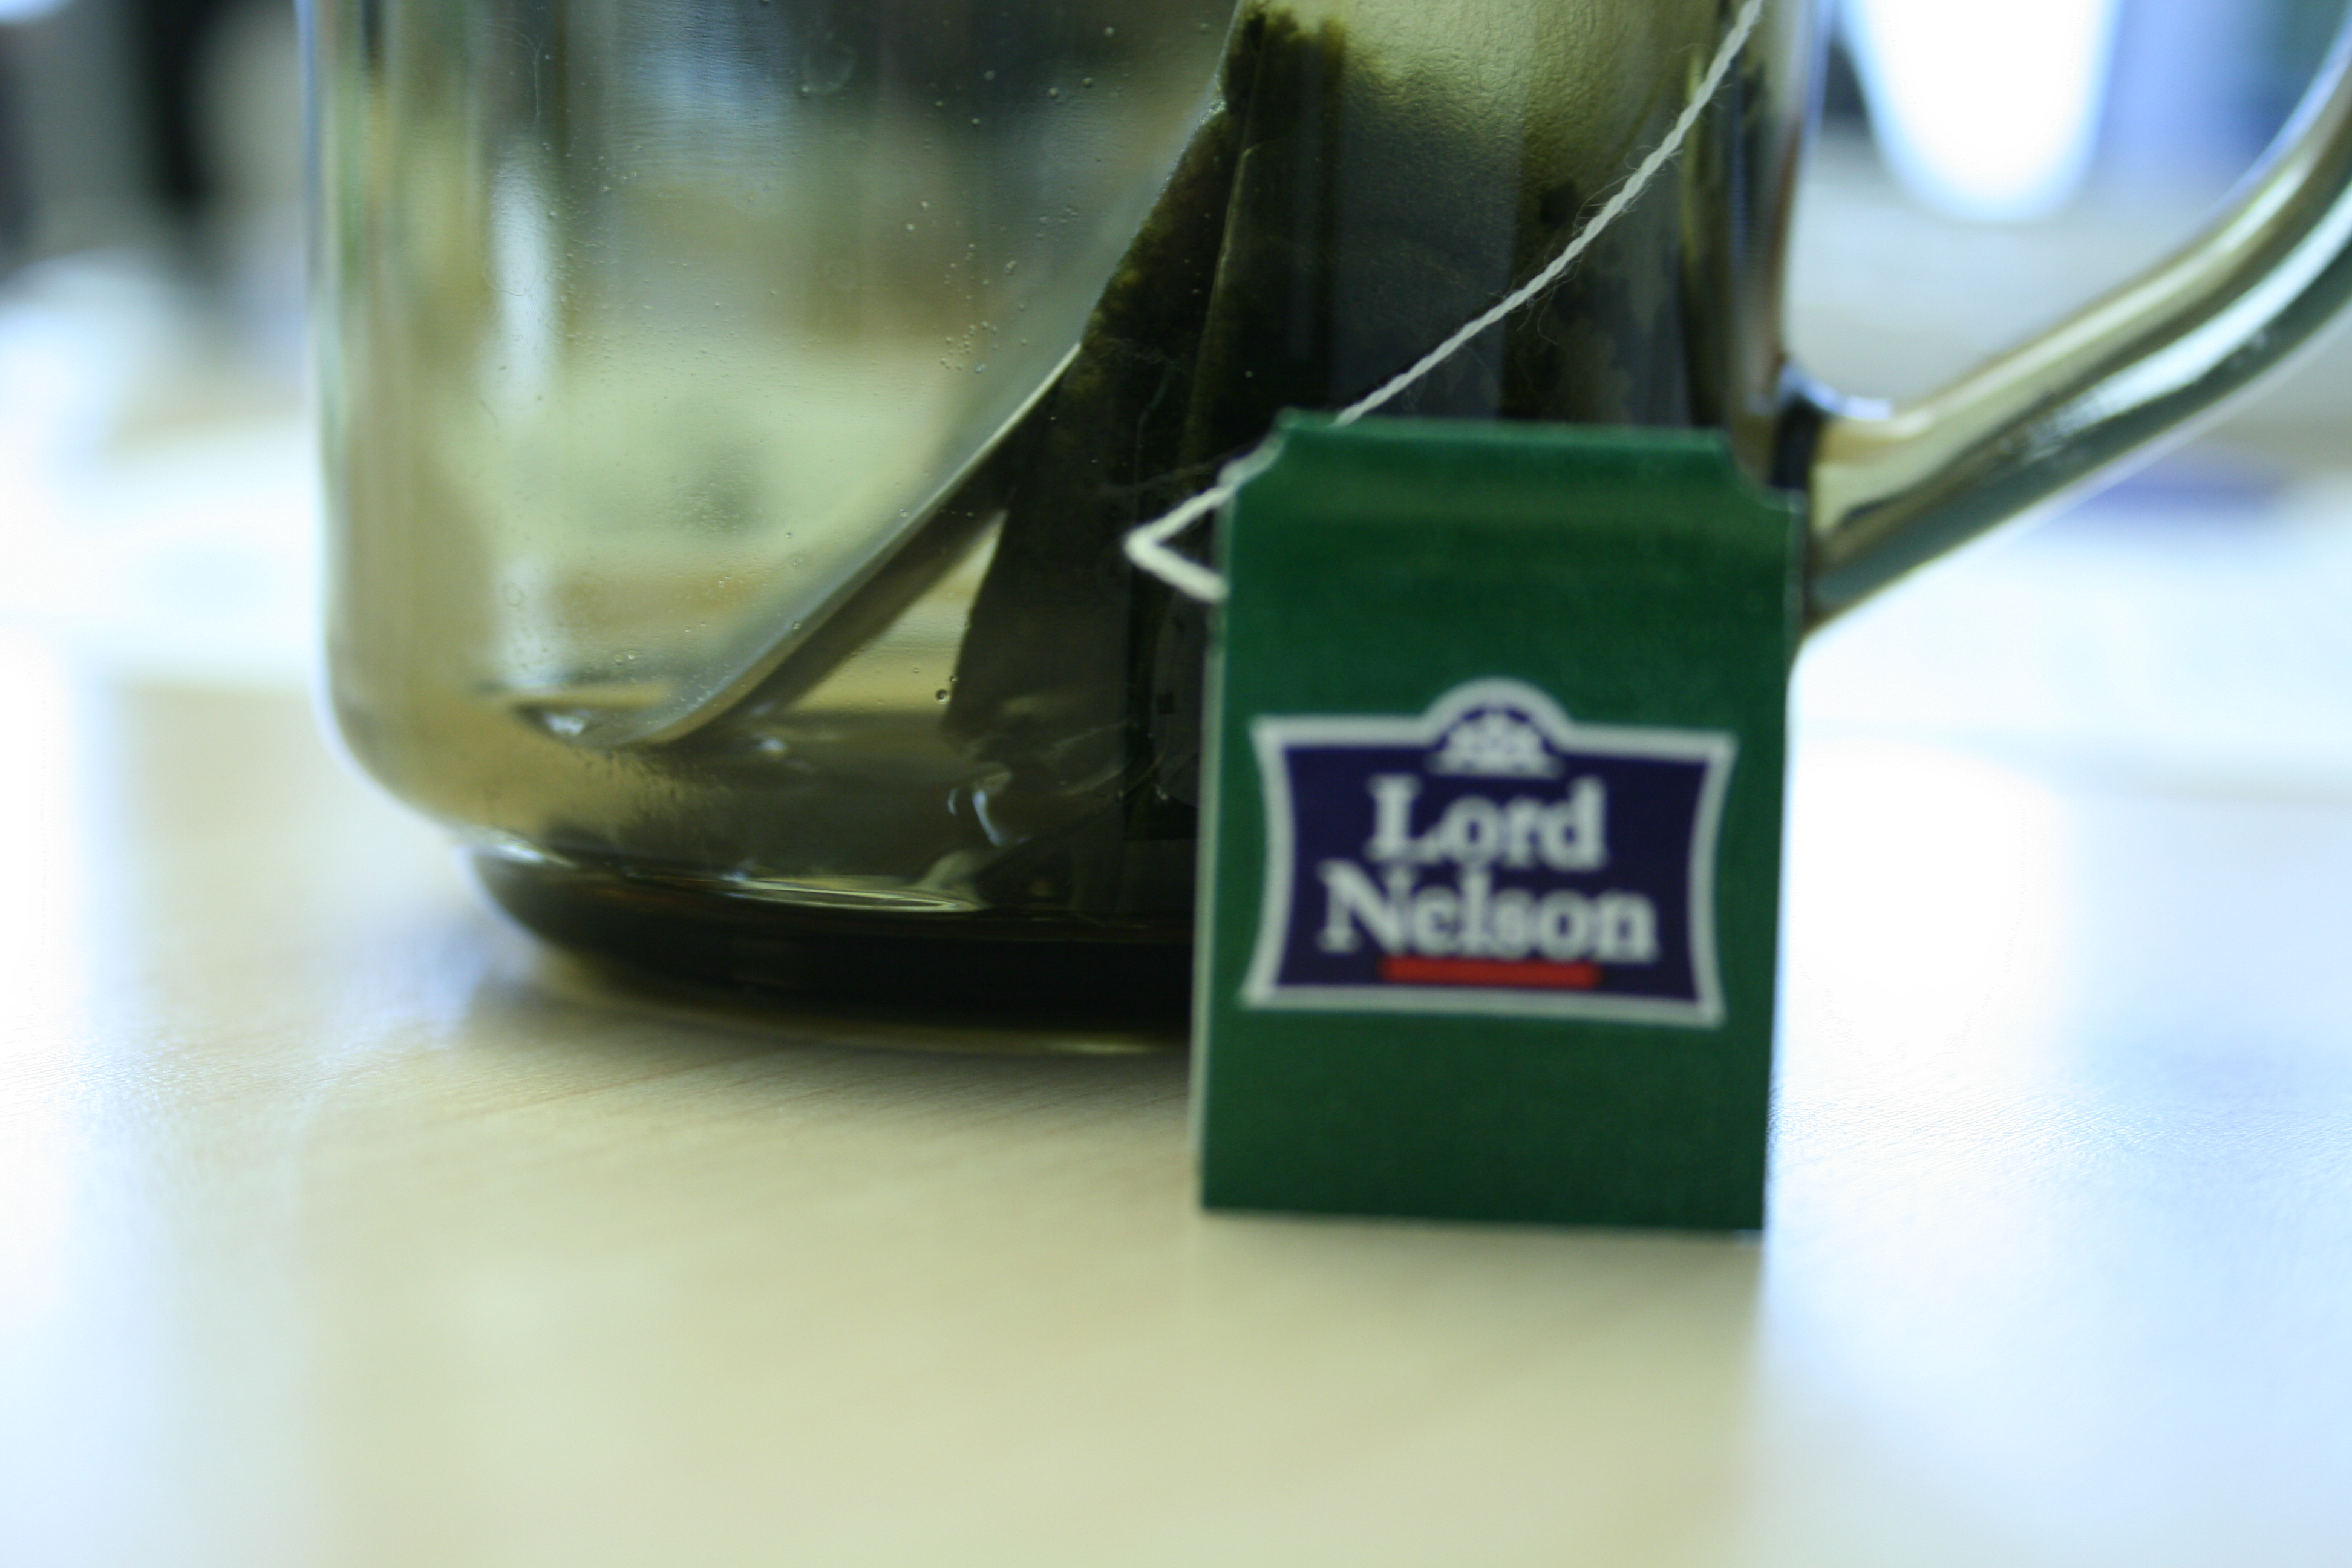
\includegraphics[height=0.172\textheight]{dataset_samples/icdar13/img_16.jpg}
    	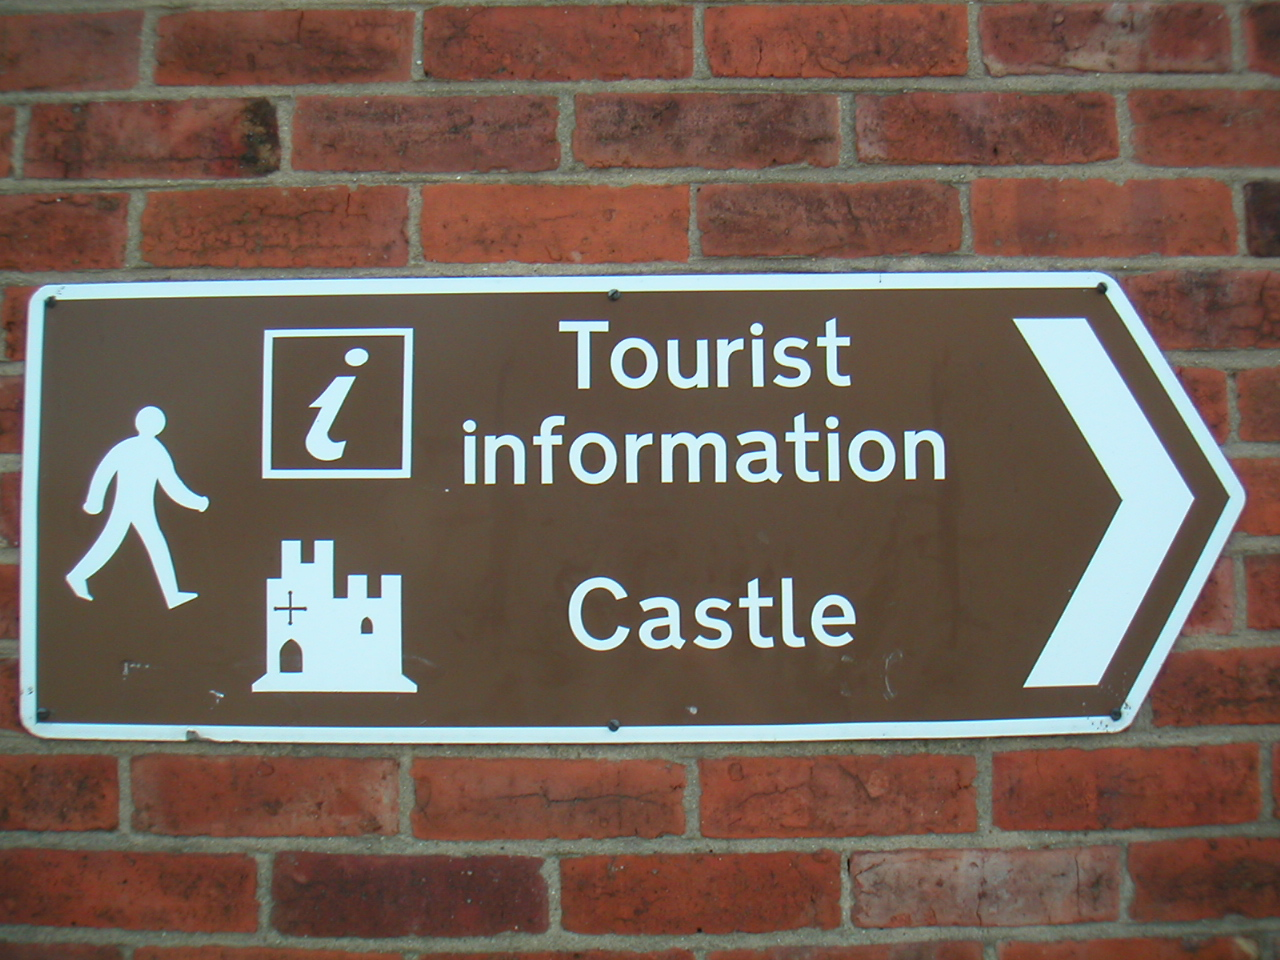
\includegraphics[height=0.172\textheight]{dataset_samples/icdar13/img_83.jpg}
    	
    	\caption{Examples of scene text images (extracted from the ICDAR'13 dataset~\cite{Karatzas2013ICDAR}).}
    	\label{fig:sample_icdar13}
    \end{figure}
    
    \subsection{Text Localization}
    The process of detecting texts present in an image is called text localization. The fundamental goal is to determine which regions of an image contain a textual element, considering the fact that there is no prior information on whether or not the input image contains any text. Found textual elements are often enclosed in bounding-boxes with as minimum background as possible, or the pixels constituting the textual element can be highlighted in a binary mask. In this process, the text in the image is segmented from the background. Figure~\ref{fig:bbox-example} shows examples of outputs of a text localization algorithm\cite{wang2011}.
   % \todo[inline]{Include one or two more example in this Figure. We have space for that.}
    \begin{figure}[h!]
        \centering
    	
\includegraphics[height=0.25\textheight]{related_work/figs/example_text_recognition.png}
    	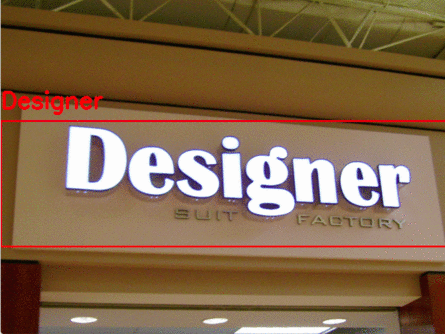
\includegraphics[height=0.25\textheight]{related_work/figs/example_text_recognition2.png}
    	\caption{Examples of bounding boxes delimiting texts in images, with the recognized words above each bounding box~\cite{wang2011}.}
    	\label{fig:bbox-example}
    \end{figure}
    
    \subsection{Text Recognition}
    The objective of the text recognition process is basically the same as those of Optical Character Recognition (OCR) software. Given input digital images or videos, the goal is to identify alphabets, numbers, punctuation marks or special characters, without any human cooperation, and then convert each of the recognized symbols into an appropriate character code. Figure~\ref{fig:bbox-example} shows the recognized characters above the bounding box of the located word. 
    
    \subsection{Text Detection and Recognition Methods}
    A common way of categorizing existing methods for text detection and recognition relies on dividing them into deep-learning and non-deep learning groups. In this work, we are assuming that a deep learning method is a machine learning apparatus so that the feature extraction and the classification modules are both trainable. The remaining methods are therefore classified as non-deep methods, even the ones with a trainable classifier but without trainable feature extraction. 
    
        %\subsubsection{Non-deep methods}
    Several non-deep methods were proposed to solve the problem of text detection and recognition. 
    One category of non-deep text detection methods is based on connected component analysis (CCA).  Being essentially a graph-based algorithm, CCA approaches take a set of connected components of the image, each one of them individually labeled by a heuristic about feature similarity. Pattern recognition methods are often used to analyze the spatial and feature consensus of the connected components and then define text regions. Some approaches~\cite{Lee2010,Kumuda2016,HyungIlKoo2013} rely on statistical models like AdaBoost to learn the CCA models, which significantly improve their robustness.  

    Another category of text detection methods consist of the sliding window classification methods. The principle of these methods is sliding a multiscale window through the image, classifying the regions defined by the sliding window as text and non-text regions. Later, positive regions are then grouped into text regions with morphological operations, conditional random fields, or graph methods~\cite{Lee2011,wang2011,Coates,Ng2011}. This class of methods is simple and adaptive. Nevertheless, they are computationally expensive when a complex classifier is used, and a large number of sliding windows needs to be classified. 
    
    Regarding the text recognition problem, a branch of proposals adopted feature-based methods. Some adopted recognition algorithms based on character segments~\cite{Shi2013,Yao}, others exploited label embedding to match strings and images directly~\cite{Rodriguez-Serrano,Gordo2014,Almazan2014}. Features like Stroke~\cite{Buta2015} and character keypoints~\cite{Phan2013} are also detected for the classification problem. The other great branch of non-deep text recognition solutions opted by decomposing the task into sub-problems, such as text binarization, text line segmentation, character segmentation, single character recognition, and word correction~\cite{Lee2013,QixiangYe,Nomura2005,Chen2004,Karatzas2004}. 
    
   The last class of methods refers to end-to-end solutions. This category of methods integrates text detection and text recognition problems into a single system responsible for both tasks. In some initiatives like~\cite{Felzenszwalb2005}, characters are treated as a special case of object detection, being detected by a Nearest Neighbor algorithm trained with shape descriptors and then grouped into words by using a model that relies on a Pictorial Structure. In another work~\cite{Neumann2013}, the authors proposed a delayed decision approach by keeping multiple segmentation samples from each character until the context of each character is known. The segmentation of detected characters was obtained using extremal regions and decoded recognition results in a dynamic programming algorithm.
        
        %\subsubsection{Deep methods}
        %This section describes some of the deep-learning-based text detection and recognition methods.
        %\textcolor{red}{Provide the meaning of the acronyms}
        %SSTD~\cite{sstd} is a variation of the SSD~\cite{ssd} architecture focused on text detection. This proposal outputs word-level bounding boxes, and can be divided into three parts: the convolutional module, the box prediction module and the text specific module. The convolutional and text specific module are directly inherited from the SSD model. The text specific module can be divided into two modules: a text attention module and a hierarchical inception module. The text attention module is responsible for learning rough spatial text features form the convolutional layers, aiming at reducing false detection, detecting more ambiguous text and improving accuracy. The hierarchical inception module has the task to aggregate multiscale features so that multiscale text can be better detected. 
        %
        %Liao et al.~\cite{textboxes} proposed a fully convolutional network adapted for text detection and recognition, named TextBoxes. The authors approach inherits the VGG16~\cite{vgg} architecture, converting the last two fully-connected layers to convolutional layers by parameter downsampling. Multiple output layers are inserted after the last and some of the intermediate layers, and their outputs are aggregated, afterwards passing in a non-maximal supression process.
        %
        %The TextBoxes approach was later extended as the TextBoxes++~\cite{textboxes++} proposal. The objective was to support the detection of arbitrary oriented bounding boxes. The proposed architecture is also a fully convolutional network. This approach extends the original proposal by predicting an arbitrary quadrilateral as a text bounding box, nos only vertically oriented boxes.
        
        %Another way to perform text detection on images relies on the use of methods originally proposed as object detection techniques. The YOLO V3~\cite{yolov3} (You Only Look Once V3) is a fully convolutional network proposed for object detection that reflects the improvements of the authors over the second version of this method. Being based on the GoogLeNet~\cite{googlenet} model, this proposal predicts bounding boxes and class probabilities directly from full images in one evaluation. The system predicts 4-coordinate bounding boxes using dimension clusters as anchor boxes and predicts an objectness score for each bounding box using logistic regression. 
      
        
        
        
   
   
   